\section{Leitura da Instrução}
	\subsection{Diagrama de Classe}
  \begin{figure}[H]
    \begin{center}
	\begin{tikzpicture}
	\umlclass[type = control]{Instruction Fetch}{
	+ clock : input bit \\
	+ reset : input bit \\
	+ pcInput : input bit[14] \\ 
	+ pcWrite : input bit \\
	+ pcOutput : output bit[14] \\
	+ instruction : output bit[32] }			
	{
	- \underline{<<comb>> search\_Instruction()} \\
	- <<comb>> next\_PC() 
	}
	\end{tikzpicture}
\end{center}
  \end{figure}
		
		\subsection{Definições de entrada e saída}
		
	\begin{center}
		\begin{longtable}[pos]{| l | c | c | m{7cm} |} \hline
			\multicolumn{1}{|c|}{\cellcolor[gray]{0.9}\textbf{Nome}} & 
			\multicolumn{1}{c|}{\cellcolor[gray]{0.9}\textbf{Tamanho}} & 
			\multicolumn{1}{c|}{\cellcolor[gray]{0.9}\textbf{Direção}} &
			\multicolumn{1}{c|}{\cellcolor[gray]{0.9}\textbf{Descrição}} \\ \hline
			\endhead
			\hline
			\endlastfoot
			
			pcInput & 32 & entrada & Valor do PC atual.\\ \hline
			pcWrite & 1 & entrada & Sinal proveniente da UC que habilita a modificação do valor de PC. \\ \hline
			pcOutput & 32 & saída & Valor do PC atual. \\ \hline
			instruction & 32 & saída & Instrução a ser executada. \\ \hline
			
		\end{longtable}
	\end{center}
	
	\subsection{Datapath Interno}
	
	\begin{figure}[ht]
		\begin{center}
		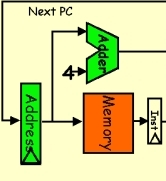
\includegraphics{./datapath/step1.jpg}
		\caption*{Datapath preliminar}
		\end{center}
	\end{figure}
